\documentclass[11pt]{article}

\usepackage[T1]{fontenc} % extended font encoding
\usepackage{enumerate} % lists
\renewcommand{\familydefault}{\sfdefault} % sans-serif
\usepackage{microtype} % better text justification
\usepackage{graphicx} % allow including pictures
\usepackage{color} % colors for pictures
\usepackage{textcomp} % for textminus
\usepackage{pagecolor} % background color for the first page
\usepackage{afterpage} % ditto ^^
\usepackage{tikz} % flow graph
\usetikzlibrary{dsp,chains}
\usepackage{parskip} % vertical paragraph spacing
\usepackage{hyperref} % links
\usepackage{tcolorbox} % boxes around text
\usepackage[a4paper, landscape, margin=1.5cm]{geometry} % basic geometry
\fboxsep=5mm % minibox spacing
\pagenumbering{gobble} % disable page numbering
\renewcommand{\thefootnote}{\arabic{footnote}} % use numbers for footnotes
\renewcommand{\thempfootnote}{\arabic{mpfootnote}} % ditto for minipages

% Style for a simple numbered list
\newenvironment{packed_enumerate}{
\begin{enumerate}
  \setlength{\itemsep}{1pt}
  \setlength{\parskip}{0pt}
  \setlength{\parsep}{0pt}
}{\end{enumerate}}

% Style for a roman literal numbered list
\newenvironment{packed_enumerate_i}{
\begin{enumerate}[I]
  \setlength{\itemsep}{1pt}
  \setlength{\parskip}{0pt}
  \setlength{\parsep}{0pt}
}{\end{enumerate}}


% Metadata
\pdfinfo{
   /Author (Zlosynth Instruments)
   /Title  (Arplus - User Manual)
}

\begin{document}

% Front page should be black
\pagecolor{black}\afterpage{\nopagecolor}

% Front title
\title{\textcolor{white}{MANUAL}}
\author{}
\date{}

% Left column of the front page
\begin{minipage}{0.4\textwidth}
\color{white}
\maketitle

% Overview box
\noindent\colorbox{white}
{
\begin{minipage}{0.85\textwidth}\color{black}
TODO About the module, what it combines and what it provides.
\end{minipage}
}

\vspace{1cm}

% Specs table
\begin{minipage}{0.8\textwidth}\color{white}
\begin{tabular}{@{}rl@{}}
  Width & 14 HP \\
  Depth & 28 mm TODO \\
  Power & +12 V (117 mA), \textminus12 V (8 mA) TODO \\
  Input impedance & 100 kΩ \\
  Trigger inputs & 0 to +5 V, 1 kHz \\
  CV inputs & \textminus5 to +5 V, 16-bit, 1 kHz \\
  CV output & \textminus0 to +5 V, 16-bit, 1 kHz \\
  Audio & 24-bit, 48 kHz
\end{tabular}
\end{minipage}

\vspace{1cm}

% Features list
\begin{minipage}{0.8\textwidth}\color{white}
\begin{tabular}{@{}l}
  - TODO: Features in a list \\
  - TODO: Features in a list \\
  - TODO: Features in a list \\
  - TODO: Features in a list
\end{tabular}
\end{minipage}

\end{minipage}%
% Right column
\begin{minipage}{0.6\textwidth}
\vspace{8mm}

% Illustration of the panel
\begin{center}
  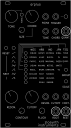
\includegraphics[width=0.55\textwidth]{diagram-panel.pdf}
\end{center}

\end{minipage}

% Start of the quick start page
\newpage
% \color{black}

% Left column

\section{Installation}

Arplus is 14 HP wide. It is powered by a +12V/{\textminus}12V 2\texttimes5
connector. The red stripe (\textminus12V) has to be connected on the side of the
board marked with the white line. The module must be mounted in a eurorack case.

\vspace{2.5cm}

\section{Signal flow}

\vspace{2.5cm}

\vspace{5mm}\begin{center}
\includegraphics[width=0.7\textwidth]{diagram-flow.pdf}\vspace{5mm}\end{center}
\newpage

\noindent\begin{tcolorbox}[
  width=0.48\textwidth,
  nobeforeafter,
  boxsep=0pt,
  left=0pt,
  right=0pt,
  top=0pt,
  bottom=0pt,
  colframe=white,
  colback=white,
  sharp corners
]

\section{Root note}

Select the root note of the playing chord. This sets the pitch of the lowest
playing tone in the arpeggio.

\vspace{2cm}

\begin{tcolorbox}[
  standard jigsaw,
  colframe=black,
  colback=white,
  sharp corners,
  title=Using potentiometer
]
  \vspace{0.5cm}
  \begin{center}
    
\includegraphics{diagram-tone-pot.pdf}
  \end{center}
  \vspace{1.0cm}
  \noindent\begin{tcolorbox}[
    standard jigsaw,
    width=.375\textwidth,
    colframe=black,
    colback=white,
    colbacktitle=white,
    coltitle=black,
    sharp corners,
    nobeforeafter,
    title=Legend
  ]
    \begin{center}
      
\includegraphics{diagram-tone-pot-led.pdf}
    \end{center}
  \end{tcolorbox}\hfill
  \begin{tcolorbox}[
    width=.575\textwidth,
    standard jigsaw,
    colframe=black,
    colback=white,
    colbacktitle=white,
    coltitle=black,
    sharp corners,
    nobeforeafter,
    title=Example
  ]
    \begin{center}
      
\includegraphics{diagram-tone-pot-led-example.pdf}
    \end{center}
  \end{tcolorbox}
\end{tcolorbox}

\end{tcolorbox}\hfill
\begin{tcolorbox}[
  width=0.48\textwidth,
  nobeforeafter,
  boxsep=0pt,
  left=0pt,
  right=0pt,
  top=0pt,
  bottom=0pt,
  colframe=white,
  colback=white,
  sharp corners
]

\begin{tcolorbox}[
  standard jigsaw,
  colframe=black,
  colback=white,
  sharp corners,
  title=Using CV
]
  \vspace{0.5cm}
  \begin{center}
    
\includegraphics{diagram-tone-cv.pdf}
  \end{center}
  \vspace{1.0cm}
  \noindent\begin{tcolorbox}[
    standard jigsaw,
    width=.375\textwidth,
    colframe=black,
    colback=white,
    colbacktitle=white,
    coltitle=black,
    sharp corners,
    nobeforeafter,
    title=Legend
  ]
    \begin{center}
      
\includegraphics{diagram-tone-cv-led.pdf}
    \end{center}
  \end{tcolorbox}\hfill
  \begin{tcolorbox}[
    width=.575\textwidth,
    standard jigsaw,
    colframe=black,
    colback=white,
    colbacktitle=white,
    coltitle=black,
    sharp corners,
    nobeforeafter,
    title=Example
  ]
    \begin{center}
      
\includegraphics{diagram-tone-cv-led-example.pdf}
    \end{center}
  \end{tcolorbox}
\end{tcolorbox}

\end{tcolorbox}

\newpage


\noindent\begin{tcolorbox}[
  width=0.48\textwidth,
  nobeforeafter,
  boxsep=0pt,
  left=0pt,
  right=0pt,
  top=0pt,
  bottom=0pt,
  colframe=white,
  colback=white,
  sharp corners
]

\section{Chord}

Select from an assorted list chords grouped by size.

\vspace{2cm}

\begin{tcolorbox}[
  standard jigsaw,
  colframe=black,
  colback=white,
  sharp corners,
  title=Setting chord size
]
  \vspace{0.5cm}
  \begin{center}
    
\includegraphics{diagram-chord-size.pdf}
  \end{center}
  \vspace{0.5cm}
  \noindent\begin{tcolorbox}[
    standard jigsaw,
    width=.375\textwidth,
    colframe=black,
    colback=white,
    colbacktitle=white,
    coltitle=black,
    sharp corners,
    nobeforeafter,
    title=Legend
  ]
    \begin{center}
      
\includegraphics{diagram-chord-size-led.pdf}
    \end{center}
  \end{tcolorbox}\hfill
  \begin{tcolorbox}[
    width=.575\textwidth,
    standard jigsaw,
    colframe=black,
    colback=white,
    colbacktitle=white,
    coltitle=black,
    sharp corners,
    nobeforeafter,
    title=Example
  ]
    \begin{center}
      
\includegraphics{diagram-chord-size-led-example.pdf}
    \end{center}
  \end{tcolorbox}
\end{tcolorbox}

\end{tcolorbox}\hfill
\begin{tcolorbox}[
  width=0.48\textwidth,
  nobeforeafter,
  boxsep=0pt,
  left=0pt,
  right=0pt,
  top=0pt,
  bottom=0pt,
  colframe=white,
  colback=white,
  sharp corners
]


  \begin{tcolorbox}[
    standard jigsaw,
    colframe=black,
    colback=white,
    sharp corners,
    title=Selecting chord
  ]
    \vspace{0.5cm}
    \noindent\begin{tcolorbox}[
      standard jigsaw,
      width=.375\textwidth,
      colframe=black,
      colback=white,
      sharp corners,
      nobeforeafter,
      title=Using potentiometer
    ]
      \begin{center}
        
\includegraphics{diagram-chord-pot.pdf}
      \end{center}
    \end{tcolorbox}\hfill
    \begin{tcolorbox}[
      width=.575\textwidth,
      standard jigsaw,
      colframe=black,
      colback=white,
      sharp corners,
      nobeforeafter,
      title=Using CV
    ]
      \begin{center}
        
\includegraphics{diagram-chord-cv.pdf}
      \end{center}
    \end{tcolorbox}
    \vspace{0.5cm}

    \noindent\begin{tcolorbox}[
      standard jigsaw,
      width=.375\textwidth,
      colframe=black,
      colback=white,
      colbacktitle=white,
      coltitle=black,
      sharp corners,
      nobeforeafter,
      title=Legend
    ]
      \begin{center}
        
\includegraphics{diagram-chord-led.pdf}
      \end{center}
    \end{tcolorbox}\hfill
    \begin{tcolorbox}[
      width=.575\textwidth,
      standard jigsaw,
      colframe=black,
      colback=white,
      colbacktitle=white,
      coltitle=black,
      sharp corners,
      nobeforeafter,
      title=Example
    ]
      \begin{center}
        
\includegraphics{diagram-chord-led-example.pdf}
      \end{center}
    \end{tcolorbox}
  \end{tcolorbox}

\end{tcolorbox}

\newpage
\noindent\begin{tcolorbox}[
  width=0.675\textwidth,
  nobeforeafter,
  boxsep=0pt,
  left=0pt,
  right=0pt,
  top=0pt,
  bottom=0pt,
  colframe=white,
  colback=white,
  sharp corners
]

\section{Arpeggio}

In arpeggio, notes of the selected chord are triggered individually. The
selected type defines how should be the notes ordered. Some types can be RESET
to their initial position. Other types are repeating the same sequence until
NEXT is triggered.

\begin{tcolorbox}[
  standard jigsaw,
  nobeforeafter,
  boxsep=0pt,
  left=0pt,
  right=0pt,
  top=0pt,
  bottom=0pt,
  colframe=white,
  colback=white,
  sharp corners
]
  \vspace{0.5cm}
  \noindent\begin{tcolorbox}[
    standard jigsaw,
    width=.48\textwidth,
    colframe=black,
    colback=white,
    sharp corners,
    nobeforeafter,
    enlarge bottom by=4cm,
    title=Selecting type
  ]
    \vspace{0.5cm}
    \noindent\begin{tcolorbox}[
      standard jigsaw,
      width=.375\textwidth,
      boxsep=0pt,
      left=0pt,
      right=0pt,
      top=0pt,
      bottom=0pt,
      colframe=white,
      colback=white,
      nobeforeafter,
      sharp corners
    ]
      \begin{center}
        
\includegraphics{diagram-arp-select.pdf}
      \end{center}
      \vspace{4mm}
    \end{tcolorbox}\hfill
    \begin{tcolorbox}[
      width=.575\textwidth,
      standard jigsaw,
      colframe=black,
      colback=white,
      colbacktitle=white,
      coltitle=black,
      sharp corners,
      nobeforeafter,
      title=Query selected
    ]
      \begin{center}
        
\includegraphics{diagram-arp-query.pdf}
      \end{center}
    \end{tcolorbox}
  \end{tcolorbox}\hfill
  \begin{tcolorbox}[
    width=.48\textwidth,
    standard jigsaw,
    colframe=black,
    colback=white,
    sharp corners,
    nobeforeafter,
    title=Progression
  ]
    \vspace{0.5cm}
    \noindent\begin{tcolorbox}[
      standard jigsaw,
      width=.48\textwidth,
      colframe=black,
      colback=white,
      sharp corners,
      nobeforeafter,
      title=Using button
    ]
      \begin{center}
        
\includegraphics{diagram-arp-progression-click.pdf}
      \end{center}
    \end{tcolorbox}\hfill
    \begin{tcolorbox}[
      width=.48\textwidth,
      standard jigsaw,
      colframe=black,
      colback=white,
      sharp corners,
      nobeforeafter,
      title=Using CV
    ]
      \begin{center}
        
\includegraphics{diagram-arp-progression-cv.pdf}
      \end{center}
    \end{tcolorbox}
    \vspace{0.5cm}

    \begin{tcolorbox}[
      standard jigsaw,
      colframe=black,
      colback=white,
      colbacktitle=white,
      coltitle=black,
      sharp corners,
      nobeforeafter,
      title=Types
    ]
      \begin{center}
        
\includegraphics{diagram-arp-progression-explanation.pdf}
      \end{center}
    \end{tcolorbox}
  \end{tcolorbox}
\end{tcolorbox}


\end{tcolorbox}\hfill
\begin{tcolorbox}[
  width=0.305\textwidth,
  nobeforeafter,
  boxsep=0pt,
  left=0pt,
  right=0pt,
  top=0pt,
  bottom=0pt,
  colframe=white,
  colback=white,
  sharp corners
]

\begin{tcolorbox}[
  standard jigsaw,
  colframe=black,
  colback=white,
  sharp corners,
  title=Reset / Next bar
]
    \vspace{0.5cm}
    \noindent\begin{tcolorbox}[
      standard jigsaw,
      width=.48\textwidth,
      colframe=black,
      colback=white,
      sharp corners,
      nobeforeafter,
      title=Using button
    ]
      \begin{center}
        
\includegraphics{diagram-arp-rsnx-click.pdf}
      \end{center}
    \end{tcolorbox}\hfill
    \begin{tcolorbox}[
      width=.48\textwidth,
      standard jigsaw,
      colframe=black,
      colback=white,
      sharp corners,
      nobeforeafter,
      title=Using CV
    ]
      \begin{center}
        
\includegraphics{diagram-arp-rsnx-cv.pdf}
      \end{center}
    \end{tcolorbox}
    \vspace{0.5cm}

    \begin{tcolorbox}[
      standard jigsaw,
      colframe=black,
      colback=white,
      colbacktitle=white,
      coltitle=black,
      sharp corners,
      nobeforeafter,
      title=Types
    ]
      \begin{center}
        
\includegraphics{diagram-arp-rsnx-explanation.pdf}
      \end{center}
    \end{tcolorbox}
\end{tcolorbox}

\end{tcolorbox}


\newpage

\section{Quantization}

\begin{center}
\begin{tabular}{@{}l|l|l|l|l@{}}
  \textbf{WES (Diatonic)} & \textbf{ARB (Maqam)} & \textbf{IND (Melakarta)} & \textbf{JPN (Japanese)} & \textbf{TSQ (Full)} \\
  Ionian & Bayati & Ratnagi (2) & Hirajoshi & Tones \\
  Dorian  & Hijaz & Rupavati (12) & In & Semitones \\
  Phrygian   & Kurd & Mayamalavagowla (15) & Insen & Quarter tones \\
  Lydian    & Nahawand & Natabhairavi (20) & Iwato & \\
  Mixolydian   & Nawa Athar & Karaharapriya (22) & Yo & \\
  Aeolian  & Rast & Sangarabharanam (29) & & \\
  Locrian   & Saba & Jalavarali (39) & & \\
      & Sikah & Gamanasrama (53) & &
\end{tabular}
\end{center}

Tonic, quantized output, on trigger, dialing the scale, few words about each
group, click vs hold.

\newpage

\section{String synthesis}

Diagram of karplus strong.

Noise, filter, loopback. Noise and filter as pictures of noise over time
and frequence response with resonance.

More diagrams of noise explaining contour and pluck (width and height)
and another for filter reson and cutoff.

Picture

CV plus parameters explained. Contour explained on picture. Resonance and
cutoff on picture, with the peak height controlled by res, cutoff moving it
left and right. Root note in one output, the rest in the other.

\newpage

\noindent
\begin{minipage}[t]{0.48\textwidth}
\setlength{\parskip}{6pt}
\section{Calibration}

Calibrate the TONE input.

\begin{packed_enumerate}
  \item While holding the RESET/NEXT button, connect a jack to the TONE CV input.
  \item The bottom 4 LEDs will light up.
  \item Play note C on the CV source and press the TRIGGER button.
  \item The top 4 LEDs will light up.
  \item Play C one octave higher and press the TRIGGER button again.
  \item Successful calibration is confirmed by double blink of all LEDs TODO.
\end{packed_enumerate}

Calibrate the QUANT. ouput.

\begin{packed_enumerate}
  \item (optional) Complete TONE input calibration.
  \item While holding the ARP select button, connect a cable between the QUANT.
    output and TONE input, then let go of the button.
\end{packed_enumerate}

\vspace{0.5cm}

\end{minipage}%
\begin{minipage}{0.04\textwidth}
\phantom{ }
\end{minipage}%
% Right column
\begin{minipage}[t]{0.48\textwidth}
\setlength{\parskip}{6pt}

\section{CV re-mapping}

CV inputs can be reconfigured to control any of the module attributes.

To change the default mapping, first enter the configuration menu by holding the
GROUP and SCALE buttons for a couple (TODO) of seconds. When the menu is opened,
the LEDs will blink in an alternating pattern.

Once in the configuration menu, turn knobs to select CV source for otherwise
CV-less (TODO) attributes:

TODO XXX Fix mapping diagram - no LEDs mean unmapped.

\noindent\begin{tcolorbox}[
  standard jigsaw,
  width=.49\textwidth,
  colframe=black,
  colback=white,
  colbacktitle=white,
  coltitle=black,
  sharp corners,
  nobeforeafter,
  title=Attribute configuration
]
  \begin{tabular}{@{}rl@{}}
    \textbf{Knob} & \textbf{Attribute} \\
    TONE & Tonic \\
    CHORD SIZE & Chord size \\
    RESONANCE & Scale group \\
    CUTOFF & Scale \\
    CONTOUR & Arp \\
    PLUCK & Pluck
  \end{tabular}
\end{tcolorbox}\hfill
\begin{tcolorbox}[
  width=.49\textwidth,
  standard jigsaw,
  colframe=black,
  colback=white,
  colbacktitle=white,
  coltitle=black,
  sharp corners,
  nobeforeafter,
  title=Legend
]
  \begin{center}
    
\includegraphics{diagram-mapping-led.pdf}
  \end{center}
\end{tcolorbox}

For example, turning CUTOFF pot to the max will make it so the CONT. CV input
will control scale attribute instead.

TODO Click XX to  save the configuration.

\section{Reset}

Calibration, CV mapping and all other attributes are persisted between restarts
of the module. To reset their values, hold the TONIC button while powering
the module on.

\section{Questions?}

You can find more information about the module on
\url{https://zlosynth.com/arplus}.

TODO: If you want custom chords or scales, text me.

\vspace{3mm}

\begin{center}
petr@zlosynth.com
\end{center}

\end{minipage}

\end{document}
